\documentclass{fancyslides} 
\usepackage[utf8]{inputenc}
\usepackage{times}

\graphicspath{{img/}}

%%% Beamer settings (do not change)
\usetheme{default} 
\setbeamertemplate{navigation symbols}{} %no navigation symbols
\setbeamercolor{structure}{fg=\yourowntexcol} 
\setbeamercolor{normal text}{fg=\yourowntexcol} 



%%%%%%%%%%%%%%%%%%%%%%%%%
%%% CUSTOMISATIONS %%%%%%
%%%%%%%%%%%%%%%%%%%%%%%%%


%%%% SLIDE ELEMENTS
\newcommand{\structureopacity}{0.75} %opacity for the structure elements (boxes and dots)
\newcommand{\strcolor}{blue} %elements colour (predefined blue; orange; green)

%%%% TEXT COLOUR
\newcommand{\yourowntexcol}{white}


%%%%%%%%%%%%%%%%%%%%%%%%%
%%% TITLE SLIDE DATA %%%%
%%%%%%%%%%%%%%%%%%%%%%%%%
\fbckg{nexus}
\newcommand{\titlephrase}{Data Warehouse}
\newcommand{\name}{Javier Bonet \\ Joel Catacora \\}
\newcommand{\affil}{Base de datos avanzada}
\newcommand{\email}{1 de abril del 2015}


\begin{document}


\startingslide %this generates titlepage from the data above

\fbckg{negro}
\begin{frame}
\pointedsl{{\LARGE Business intelligence}}
\end{frame}

\fbckg{negro}
\begin{frame}
\misc{El término "\textbf{Business Intelligence}" fue acuñado originalmente por Richard Millar Devens en 'Cyclopædia of Commercial and Business Anecdotes'en 1865. Devens utilizó el término para describir cómo el banquero, Sir Henry Furnese, obtuvo beneficios por recibir y procesar la información sobre su entorno, antes que sus competidores.
\newline

La inteligencia de negocios, tal como se entiende, hoy en día se dice que ha evolucionado desde los sistemas de apoyo a las decisiones (DSS), que se inició en la década de 1960 y desarrolló a mediado de los años 80's.
}
\end{frame}

\fbckg{negro}
\begin{frame}
\misc{Se denominada \textbf{Business intelligence} (BI), al conjunto de estrategias que integran, por un lado el almacenamiento, y
por el otro, el procesamiento de grandes cantidades de datos, con el principal objetivo de
transformarlos en conocimiento y en decisiones en tiempo real, a través del análisis de los datos existentes en una organización o empresa.

\begin{center}
Dato + Análisis = Conocimiento.
\end{center}
}
\end{frame}


\fbckg{negro}
\begin{frame}
\pointedsl{{\large ¿Qué es un Data Warehouse?}}
\end{frame}


\fbckg{negro}
\begin{frame}
\misc{
Definición en términos de las características del DW:
\newline

\textbf{Data Warehouse} (DW o DWH), es una colección de datos orientada a un ámbito determinado, integrado, no volátil y variable en el tiempo, que ayuda a la toma de decisiones en la entidad en la que se utiliza.
}
\end{frame}

\fbckg{negro}
\begin{frame}
\misc{
Una definición más amplia que la anterior:
\newline

Un \textbf{Data Warehouse}, es un sistema que extrae, limpia, ajusta, y entrega los
datos de origen en un almacén de datos dimensional, y luego apoya e implementa
consultas y análisis, con el propósito de la toma de decisiones.}
\end{frame}

\fbckg{negro}
\begin{frame}
\pointedsl{Características}
\end{frame}

\fbckg{negro}
\begin{frame}
\itemized{
\item \textbf{Integrado}: Se integran datos provenientes de múltiples fuentes, posiblemente distintas.
}
\end{frame}

\fbckg{negro}
\begin{frame}
\itemized{
\item \textbf{Integrado}: Se integran datos provenientes de múltiples fuentes, posiblemente distintas.
\item \textbf{No volátil}: Una vez almacenados los datos en el DW, la información que éstos representan no debe perderse.
}
\end{frame}

\fbckg{negro}
\begin{frame}
\itemized{
\item \textbf{Integrado}: Se integran datos provenientes de múltiples fuentes, posiblemente distintas.
\item \textbf{No volátil}: Una vez almacenados los datos en el DW, la información que éstos representan no debe perderse.
\item \textbf{Variable en el tiempo}: La información histórica se mantiene en el DW a lo largo del tiempo.
}
\end{frame}

\fbckg{negro}
\begin{frame}
\pointedsl{Arquitectura}
\end{frame}

\fbckg{negro}
\begin{frame}
\begin{center}
\misc{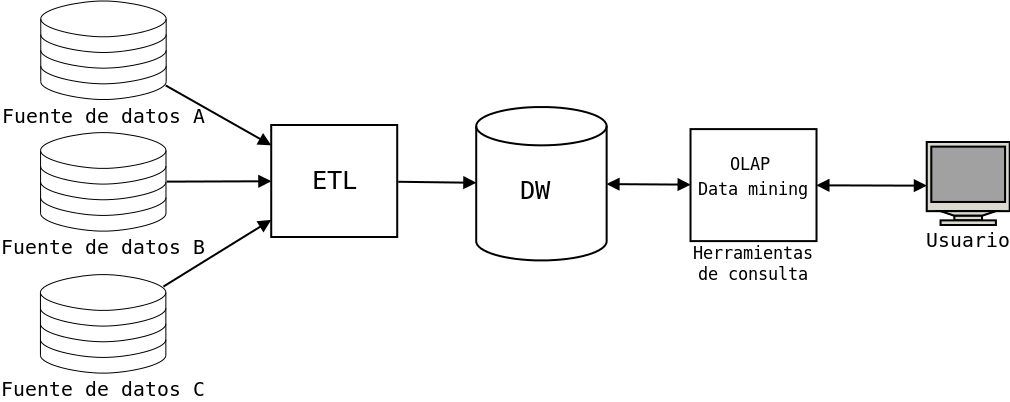
\includegraphics[scale=0.3]{arquitectura}}
\end{center}
\end{frame}

\fbckg{negro}
\begin{frame}
\pointedsl{OLTP vs. DW}
\end{frame}

\fbckg{negro}
\begin{frame}
\misc{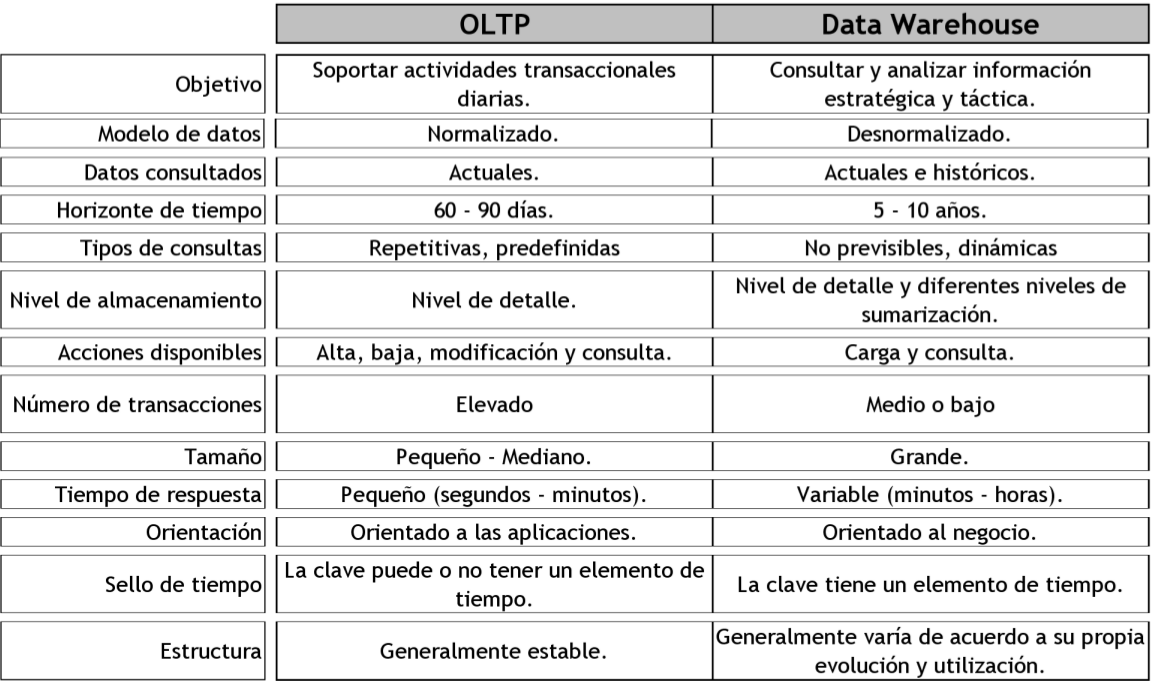
\includegraphics[scale=0.27,center]{OltpVSDW}}
\end{frame}

\fbckg{negro}
\begin{frame}
\pointedsl{Data mart}
\end{frame}

\fbckg{negro}
\begin{frame}
\misc{Los \textbf{Data marts} (DM), son subconjuntos de datos de un data warehouse para áreas específicas.

Entre las características de un data mart destacan:
\begin{itemize}
  \item Usuarios limitados.
  \item Área específica.
  \item Tiene un propósito específico.
  \item Tiene una función de apoyo.
\end{itemize}
}
\end{frame}

\fbckg{negro}
\begin{frame}
\pointedsl{{\LARGE Metodologías de diseño}}
\end{frame}

\fbckg{negro}
\begin{frame}
\misc{\textbf{Top-Down}: primero se define el DW y luego se desarrollan, construyen y cargan los
DM a partir del mismo.
\newline

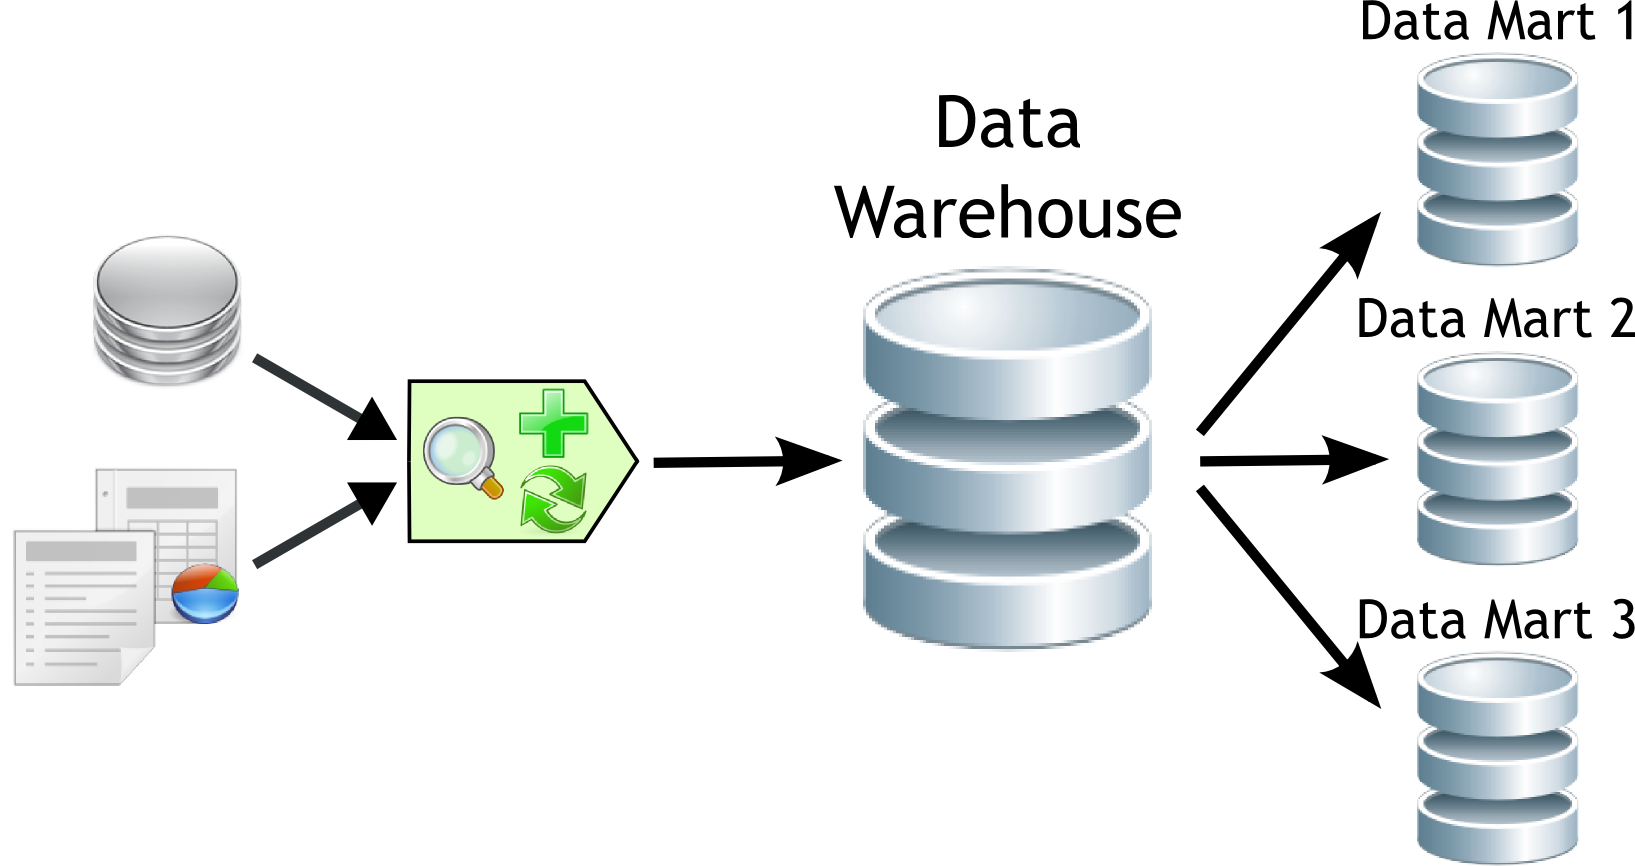
\includegraphics[scale=0.16,center]{Top-Down}
}
\end{frame}

\fbckg{negro}
\begin{frame}
\misc{\textbf{Bottom-Up}: se definen previamente los DM y luego se integran
en un DW centralizado.
\newline

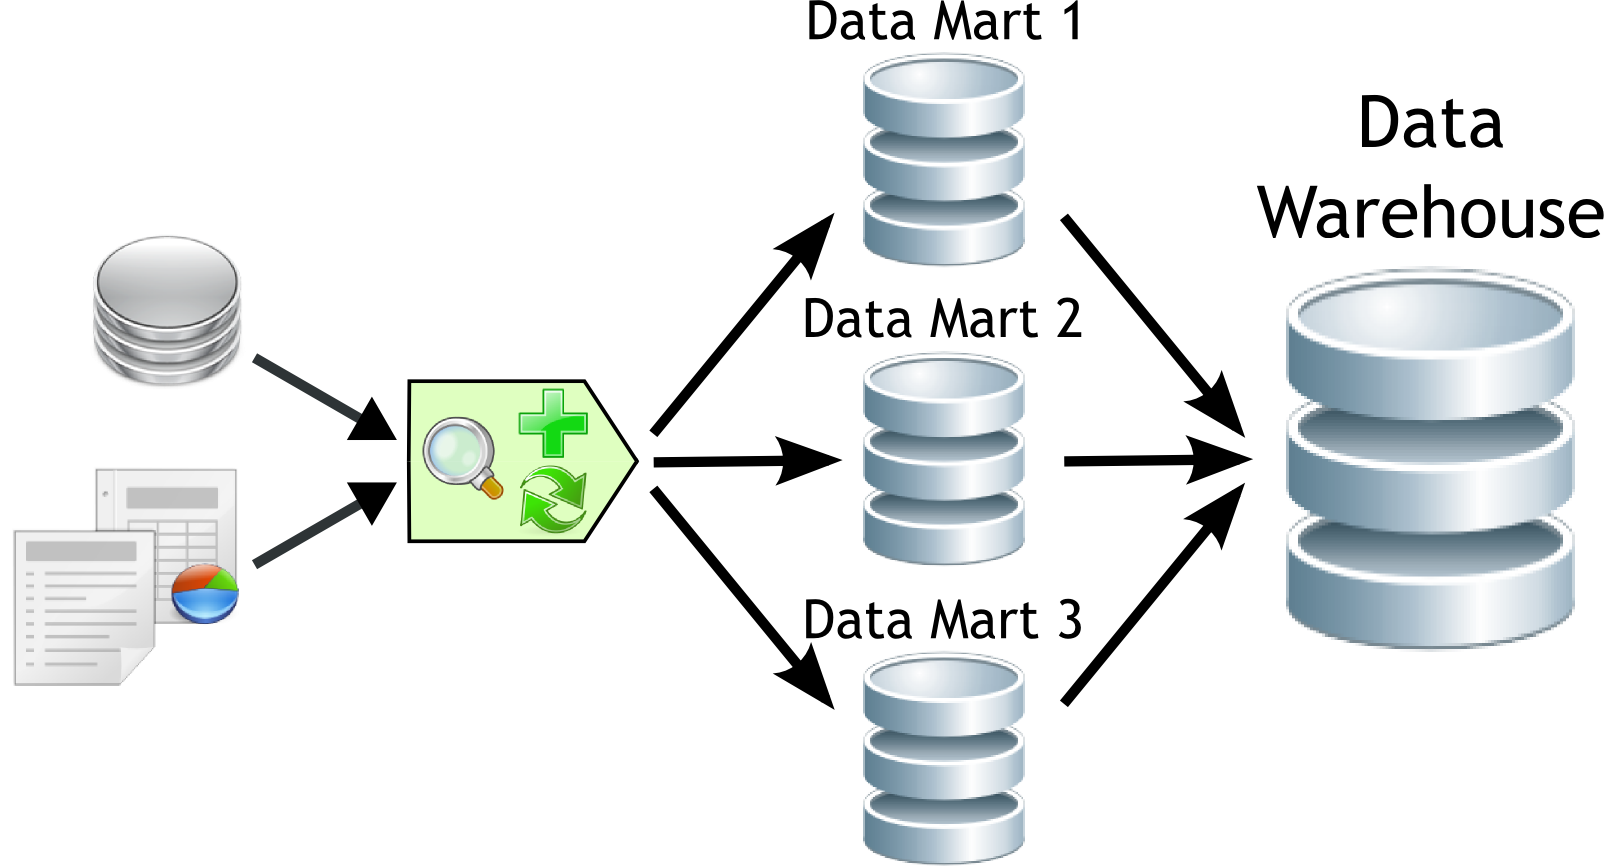
\includegraphics[scale=0.16,center]{Bottom-Up}
}
\end{frame}

\fbckg{negro}
\begin{frame}
\pointedsl{{\LARGE Modelo dimensional}}
\end{frame}

\fbckg{negro}
\begin{frame}
\misc{El modelado dimensional es una técnica de diseño lógico de una base de datos, útil para el procesamiento analítico en línea (OLAP), que tiene como ideas centrales el rendimiento y lograr la facilidad de comprensión para el usuario.
\newline

Hay dos conceptos básicos, centrales e importantes:
\begin{itemize}
  \item Hechos (métricas).
  \item Dimensiones.
\end{itemize}
}

\end{frame}

\fbckg{negro}
\begin{frame}
\pointedsl{{\LARGE Esquema dimensional}}
\end{frame}

\fbckg{negro}
\begin{frame}
\misc{Sabemos que la relación entre todas las tablas de una base de datos se denomina esquema de base de datos. Para un cierto grupo de bases de datos, en las cuales se realizan consultas sobre datos históricos, generalmente se utilizan diseños llamados esquemas dimensionales.
\newline

Un \textbf{esquema dimensional} separa físicamente las medidas que cuantifican el negocio (hechos) de los elementos que los describen (dimensiones).
}
\end{frame}

\fbckg{negro}
\begin{frame}
\misc{\textbf{Esquema estrella}
\newline


En este tipo de esquemas idea central es tener,


\textbf{Tabla de hechos}

rodeada de

\textbf{Tablas de dimensiones}
}
\end{frame}

\fbckg{negro}
\begin{frame}
\misc{\textbf{Esquema estrella}
%Supongamos que queremos realizar un análisis sobre el importe ganado por cliente, según el producto y para una fecha específica.

\begin{center}
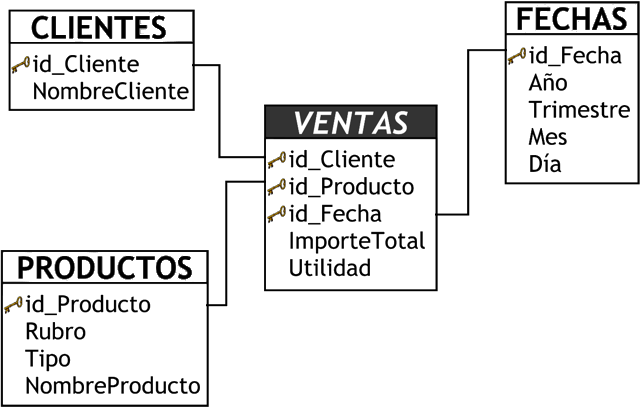
\includegraphics[scale=0.7]{Esquema_Estrella}
\end{center}
}
\end{frame}

\fbckg{negro}
\begin{frame}
\misc{\textbf{Esquema de copo de nieve}
\newline

Este otro tipo de esquemas, es similar al esquema de estrella, salvo que las dimensiones pueden estar conectadas con otras tablas de dimensiones.

Tendremos,


\textbf{Tabla de hechos}

rodeada de 

\textbf{Tablas de dimensiones}

conectadas con

\textbf{Nuevas tablas de dimensiones}
}
\end{frame}

\fbckg{negro}
\begin{frame}
\misc{\textbf{Esquema de copo de nieve}

\begin{center}
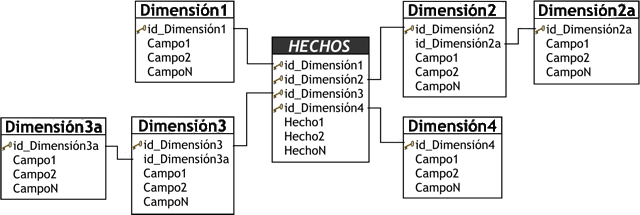
\includegraphics[scale=0.5]{copoNieve}
\end{center}
}
\end{frame}

\fbckg{negro}
\begin{frame}
\misc{\textbf{Esquema de constelación}
\newline

Este esquema es una combinación de los dos anteriores, utiliza lo mejor de cada uno, la simplicidad del esquema estrella junto con el cierto nivel de normalización del esquema copo de nieve. Está compuesto de la siguiente forma:

\textbf{Una o más tablas de hechos}

rodeada de

\textbf{Tablas de dimensiones}

conectadas (posiblemente) con

\textbf{Nuevas tablas de dimensiones}
}
\end{frame}

\fbckg{negro}
\begin{frame}
\misc{\textbf{Esquema de constelación}

\begin{center}
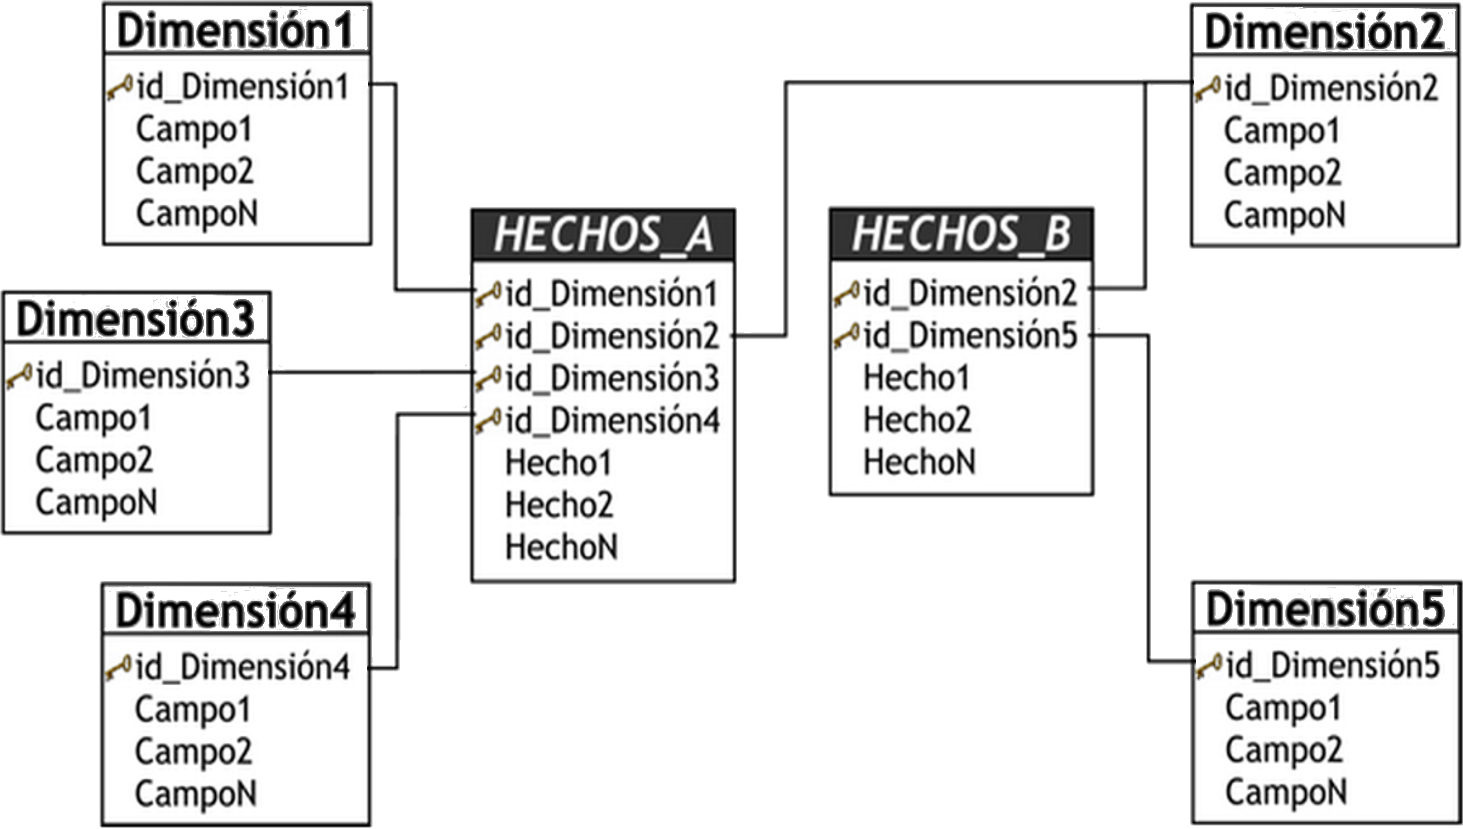
\includegraphics[width=8cm,height=8cm,keepaspectratio]{esquema_constelacion}
\end{center}

}
\end{frame}


% \begin{frame}
% \pgfsetfillopacity{1}
% 
% 
% \def\FrameCommand{\fboxsep=0cm \colorbox{\strcolor}} \MakeFramed {\FrameRestore}
% some test text
% some test text
% \endMakeFramed
% 
% \end{frame}


% \fbckg{blank}
% \begin{frame}
% \framedsl{\pitem{pointed slogan} \pitem{framed slogan} \fitem{beamer features}}
% \end{frame}
% 

% \fbckg{blank}
% \begin{frame}
%   \thankyou   %%%% ending slide with thank you notice
% \end{frame}


% \fbckg{blank}
% \begin{frame}
% \sources{
% \includegraphics[scale=0.048]{1} \ flickr/lovelornpoets\\
% \includegraphics[scale=0.2]{2} \ flickr/apsmuseum
% }
% \end{frame}

\end{document}
